\documentclass[15pt]{article}
\title{Voronoi Tessellations}
\author{stochastic13}
\date{\today}
\usepackage{graphicx}
\usepackage{subcaption}
\usepackage[margin=0.5in]{geometry}
\begin{document}
\maketitle
\tableofcontents
\newpage
\section{General working}
The script takes an input image, converts it into a \texttt{numpy} array for further processing. There are several ways to initialize the clusters for which the Voronoi maps will be computed - random (default), based on a predefined cluster-map (x,y) or a predefined probability map. Following this, the script computes distances for each pixel to all the cluster centers and picks the least distance and assigns that cluster to it (like in k-means). This is followed by either averaging of RGB channels for each cluster or exchange of channels as specified by options. The two methods to compute the actual maps are \texttt{low\_ mem} and \texttt{fast}.

\section{Syntax}
The function \texttt{VoronoiMain.py} is called in the terminal with additional options.
\begin{verbatim}

VoronoiMain.py [-h] [--rescale RESCALE] [--border BORDER]
                  [--method METHOD] [--threshold THRESHOLD]
                  [--clusmap CLUSMAP] [--probmap PROBMAP]
                  [--channel {r,g,b,rand,rb,rg,bg,randdual}]
                  [--verbose VERBOSE] [--seed SEED]
                  [--gaussianvars [GAUSSIANVARS [GAUSSIANVARS ...]]]
                  input output cn

positional arguments:
  input                 Input Image file
  output                Output Image file
  cn                    Number of clusters

optional arguments:
  -h, --help            show this help message and exit
  --rescale RESCALE     Rescaling factor for large images
  --border BORDER       Make border [1/0]?
  --method METHOD       fast vs low_mem methods. Default is low_mem.
  --threshold THRESHOLD
                        Only for borders. Threshold distance.
  --clusmap CLUSMAP     Load a specific cluster map as tab-separated text file
  --probmap PROBMAP     Load a 2D probability map for cluster generation
  --channel {r,g,b,rand,rb,rg,bg,randdual}
                        Whether to tessellate along only R,G,B or
                        combinations?
  --verbose VERBOSE     Print progress?[1/0]
  --seed SEED           Seed for PRNG
  --gaussianvars [GAUSSIANVARS [GAUSSIANVARS ...]]
                        Only for gaussian probmap
                        (mx,my,sigmax,sigmay,corr(opt),spacing(opt))
\end{verbatim}
\newpage
\section{Options}
\subsection{Required Arguments}
The three positional arguments are required to run the program. All other options are optional.
\begin{description}
\item [input] Full path (or just the name for files in the same directory) to the input image file readable by \texttt{Image.open} command in \texttt{PIL}.
\item [output] Full path (or just the name for files in the same directory) to the output file. The file will be saved as a \texttt{.jpg} file
\item [cn] The number of cluster centres. \textbf{Not all clusters will have pixel membership at the end}. Furthermore, when using \texttt{probmaps}, if the cluster lies outside the image region, it is still a valid cluster but might not have any membership. For explicitly loaded cluster maps, try to keep the clusters within the image region.
\end{description}
\subsection{Method}
There are two methods available to compute Voronoi memberships. \textbf{Default method is \texttt{low\_ mem}}. The option can be specified as \texttt{fast} or \texttt{low\_ mem} following the \texttt{--method} option.
\begin{description}
\item [low\_ mem] This takes the input array and the cluster centres, initializes an empty array the size of the image and iterates over all the pixels to compute their membership. It uses a simple nested-for loop structure and is not vectorised, and hence, slow. But this occupies significantly less memory than the other option which makes this the default choice. \emph{The progress is printed if \texttt{verbose} command is set. The printing uses a carriage-return symbol to print live percentages, which may not give the desired output in Linux, Mac or many other terminals.} The averaging of the RGB values after cluster membership computation is also slow in this process, but requires less memory.
\item [fast] This takes the input array and the cluster centers, initializes an empty array the size of the image and uses a parallel processing-based code to compute the distances and the memberships with the \texttt{multiprocessing} module. It is faster than the above method but uses significantly higher memory (see stats at the end). The averaging step is also significantly faster. The number of processes spawned depend on the default setting of the \texttt{Pool} command in \texttt{multiprocessing} module, which depends on the number of cores in the CPU.
\end{description}
\subsection{Cluster-maps}
A custom clustermap can be loaded by providing the file name to \texttt{--clusmap} option. The file must have y-values in column 1 and x-values in column 2 with tab-separated columns (the apparent inverted ordering is because the first column represents the axis=0). Try to keep the clusters in the image region since the algorithm accepts outside-region centers which may give weird results, especially when rescaling the image.
\subsection{Probability-maps}
Instead of the custom clustermaps, probability maps can also be loaded to allow for center initialization according to that probability. An inbuilt function converts the probability map into a Cumulative Distribution Function and applies Inverse Transform Sampling to sample from this distribution using a uniform random distribution (\texttt{numpy.random.rand}). The functions are custom coded and hence slow, inefficient and probably only moderately accurate. :)

An inbuilt function to have a multivariate (2-dimensional) gaussian distribution of the probabilities is also available via the \texttt{--gaussian} option. The algorithm first generates a probability array using the following:
$$p = \frac{1}{2\pi \sigma_x\sigma_y\sqrt{1-c^2}}\exp{\frac{-1}{2-2c^2}\left[\frac{(x-mx)^2}{{\sigma_x}^2}+\frac{(y-my)^2}{{\sigma_y}^2}-\frac{2c(x-mx)(y-my)}{\sigma_x\sigma_y}\right]}$$
\texttt{mx},\texttt{my},\texttt{c},\texttt{sigma} are the means for x and y, the correlation, and the sd for either respectively.
\begin{description}
\item [probmap] An input 2D array with probabilities at different points. The size is free and will be coerced to the size of the image internally. The file must have tab separated columns and newline separated rows. The values will be normalized internally, and are not needed to sum to 1. Given a uniform random number, first a marginal distribution of x is computed from which a marginal CDF of x allows inverse transform sampling to get x. Given a x, the probability distribution of y given x is used to get the corresponding CDF and y. Currently, matching the random uniform variable to the CDF value is done without any interpolation, i.e. the closest value available in the given array is chosen. Hence, larger the array, more accurate the sampling. But larger arrays might cause memory problems. Enter \texttt{gaussian} to use the internal gaussian function to generate the cluster centres.
\item [gaussianvars] Allows changing the mx,my,sigmax,sigmay,correlation,spacing for the inbuilt gaussian function. Ignored unless the \texttt{probmap} is set to \texttt{gaussian}. \texttt{spacing} is used to generate the size of the probability array and is directly put into \texttt{numpy.linspace} to generate x and y, followed by \texttt{numpy.meshgrid} before feeding into the equation.
\end{description}
\subsection{Channels}
This allows more complicated averaging once the clusters have been computed. Several options are available.
\begin{description}
\item [r,g,b] Any of these options averages only one of these channels. Each cluster has 50\% chance to be averaged and 50\% chance to stay unchanged
\item [rg,rb,bg] Each of these options exchanges the values of different channels, eg. rg exchanges the red-green channel values in half of the clusters at random. Only available with the \texttt{low\_ mem} method.
\item [rand] For each cluster, randomly averages one of the channels.
\item [randdual] For each channel, randomly exchanges any two channels. Can also keep the cluster unchanged. Only available with the \texttt{low\_ mem} method.
\end{description}
\subsection{Border}
This allows computing black borders of the clusters. Currently, a border point is a point for which the difference in distances to the closest two clusters is less than the \texttt{threshold} value. This creates uneven sized borders but in a more geometrically regular sense. More options in future versions perhaps!(Only available with the \texttt{low\_ mem} method.)
\begin{description}
\item[border] Set 1 for true. Default is 0 for false
\item[threshold] Threshold value. Coerced to int internally
\end{description}
\subsection{Other Options}
\begin{description}
\item[verbose] Whether to print messages on the standard output or no. 1 for true,0 for false. Default is true. The percentage progress uses a carriage return character to allow for printing the next update on the same line. This may cause this printing to not function properly in some systems.
\item[rescale] The input image is rescaled by this factor.
\item[seed] The seed for the Pseudo Random number generator. Fed to \texttt{numpy.random.seed}. 
\end{description}
\newpage
\section{GUI}
The GUI support has been added to make custom cluster maps. It allows the user to add the cluster centers on the image to be tessellated. The current file runs using \texttt{tkinter} library, which is the native GUI python library for \textbf{windows}. A better cross-platform support is yet to be implemented.
The utility is activated by running the \texttt{gui\_ clusmap.py} in the terminal with only two arguments, \textbf{input file} and the \textbf{output file}. The workings of the GUI are fairly intuitive, and are described below:
\begin{description}
\item [Dot Mode] Here, on clicking on the image, a single cluster center is added at the click location. Useful for very fine cluster center placements.
\item [Gaussian Spray] Allows using a spray with a Gaussian kernel to \emph{spray} the centers with the center as the Gaussian mean and the SD decided by the scale labelled \texttt{SD for spray}. Furthermore, each click adds a number of centers as selected with the slider titled \texttt{no. per click}.
\item [Add Uniform Random] This allows adding a particular number of cluster centers (as per the \texttt{no. of points to add} slider), distributed with a uniform probability distribution across the image.
\item [Reset] Resets all the centers
\item [Save] Saves the centers as a tab-separated text file, as is required by the \texttt{VoronoiMain.py} file and quits the GUI.
\end{description}
\newpage
\section{Testing}
For each of the following test, an image of size \textbf{1728 x 2304 pixels}, and ran on a \textbf{i7-8th Gen Acer Predator Helios 300 with 16GB RAM}. $t_{clus}$ represents the time in seconds for the cluster computation step, $t_{avg}$ the time for the averaging step in seconds and the max memory represents the maximum RAM memory used in MB (not very reliable, but approximately true). The seed is 123 wherever applicable. lm stands for \texttt{low\_ mem} and f stands for fast methods.

\bigskip
\bigskip
\centering
\begin{tabular}{c | c | c | c}
\textbf{Options} & $t_{clus}$ & $t_{avg}$ & max memory\\
\hline
cn 1000 rescale 2 lm & 9 & 8 & 30\\
cn 1000 rescale 2 f & 4 & 4 & 394\\
\hline
cn 500 border lm & 143 & 20 & 47\\
\hline
clusmap A lm & 48 & 63 & 50\\
clusmap A f & 16 & 8 & 751\\
\hline
cn 1000 channel r lm & 37 & 13 & 51\\
cn 1000 channel r f & 13 & 5 & 754\\
\hline
cn 500 gaussian lm & 28 & 17 & 98\\
cn 500 gaussian f & 11 & 4 & 930\\
\hline
cn 2000 probmap B lm & 50 & 51 & 50\\
cn 2000 probmap B f & 14 & 5 & 760\\
\end{tabular}
\newpage
\section{Samples}
\begin{figure}[h!]
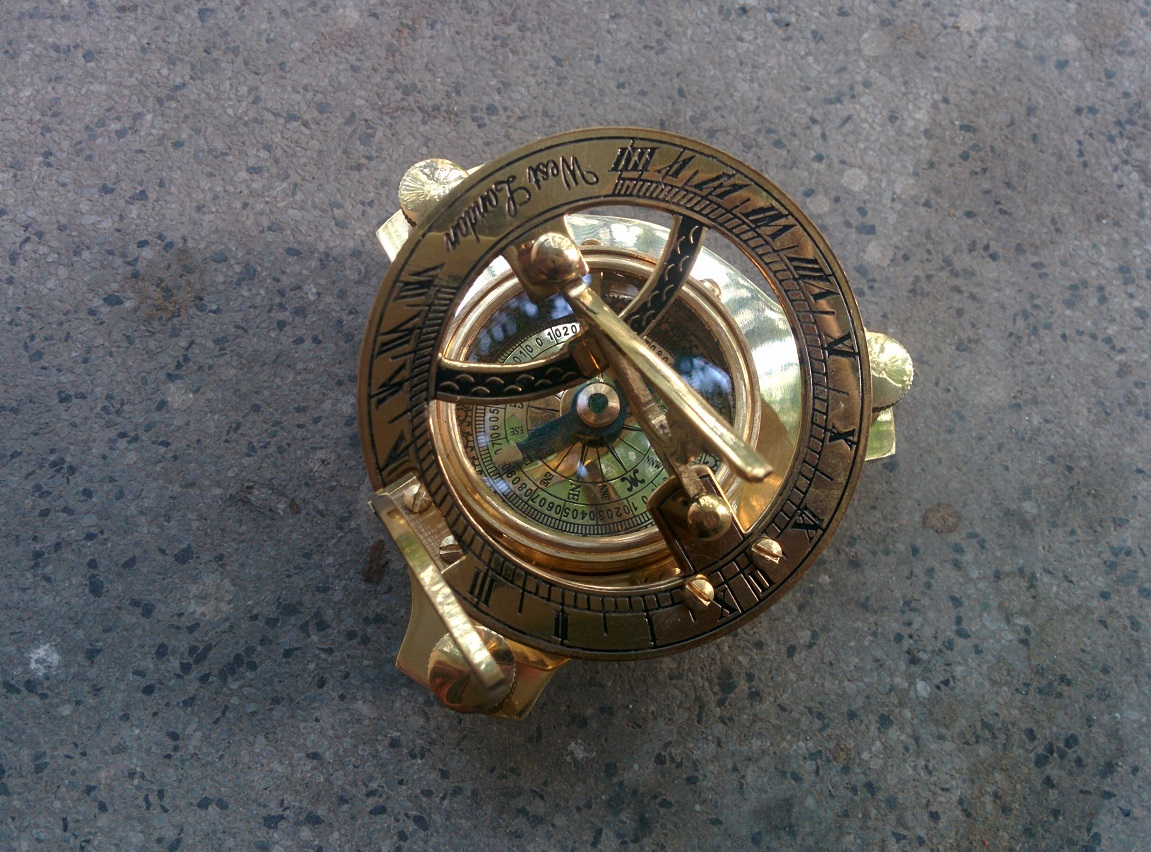
\includegraphics[width=1\linewidth]{original.jpg}
\caption{original source image}
\end{figure}
\begin{figure}
\centering
\begin{subfigure}[b]{0.48\linewidth}
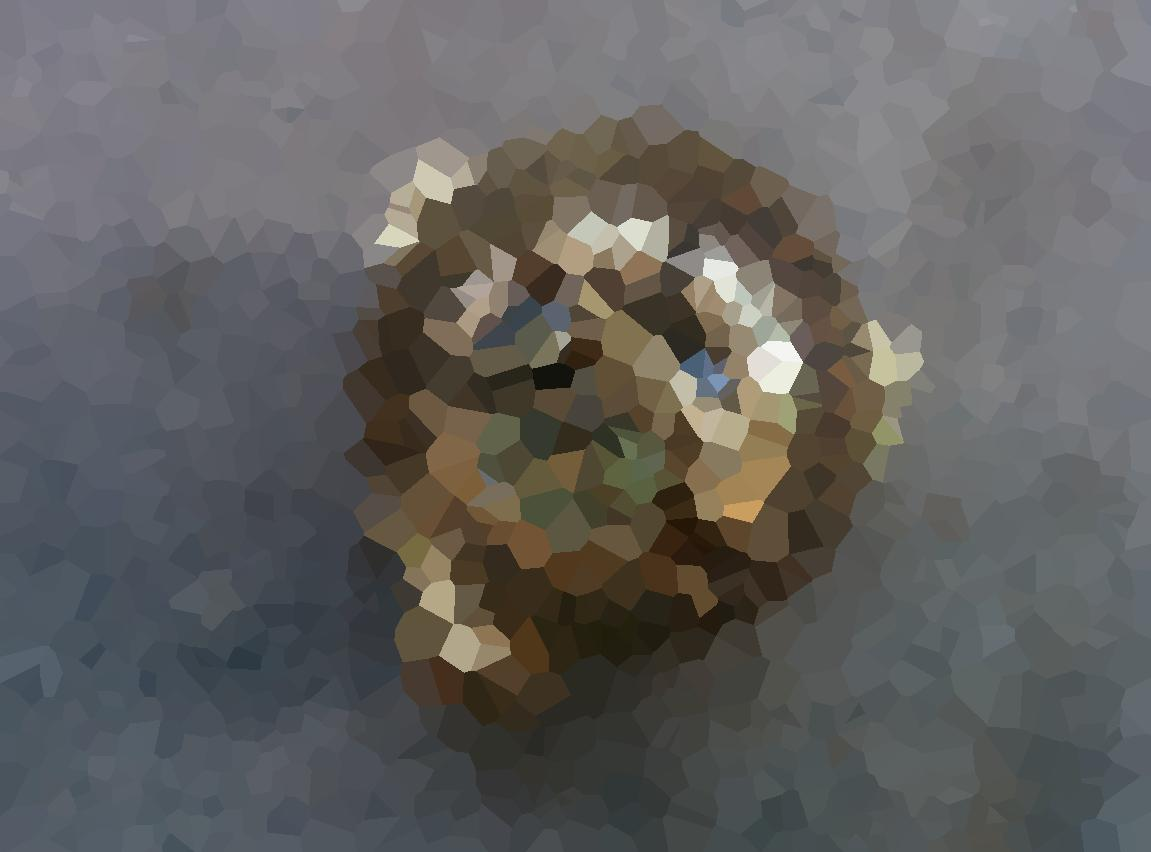
\includegraphics[width=\linewidth]{auto1500_f_s123.jpg}
\caption{cn=1500, seed=123, fast}
\end{subfigure}
\begin{subfigure}[b]{0.48\linewidth}
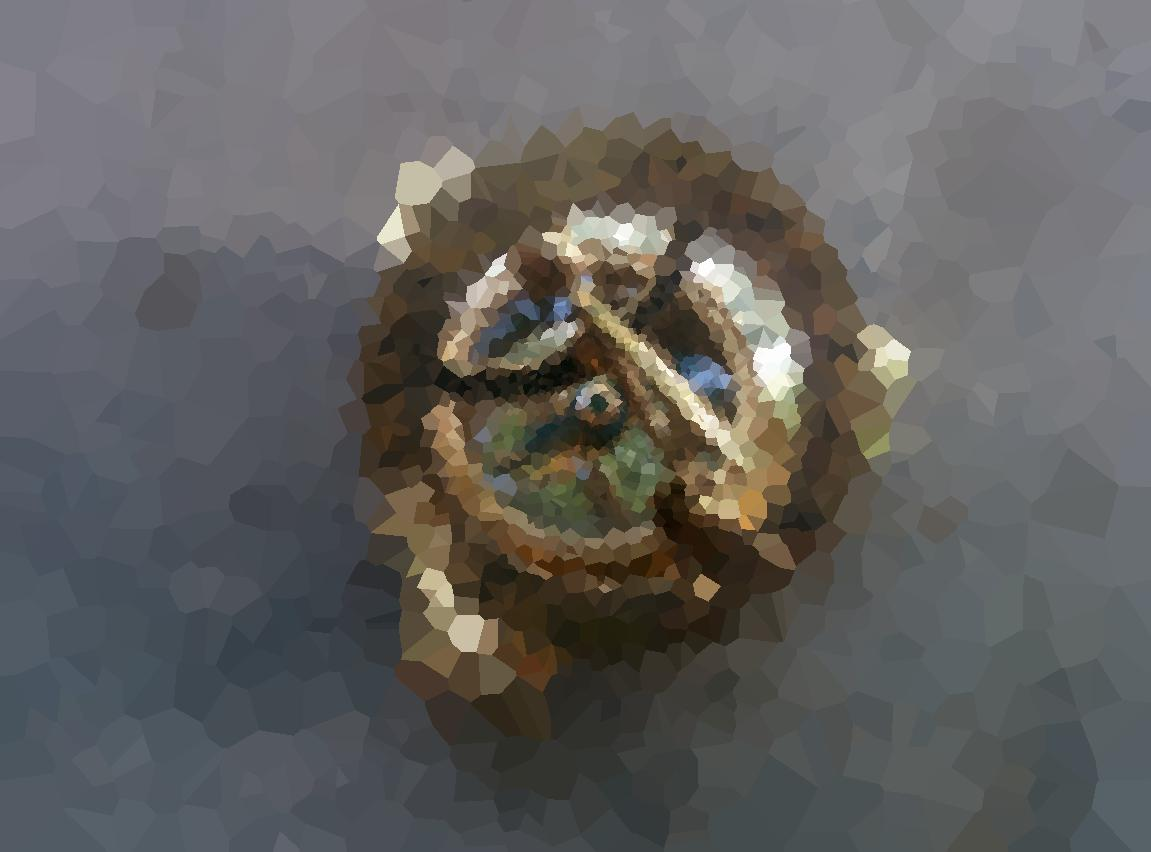
\includegraphics[width=\linewidth]{clusmap_f_s123.jpg}
\caption{demo\_ clusmap, seed=123, fast}
\end{subfigure}
\begin{subfigure}[b]{0.48\linewidth}
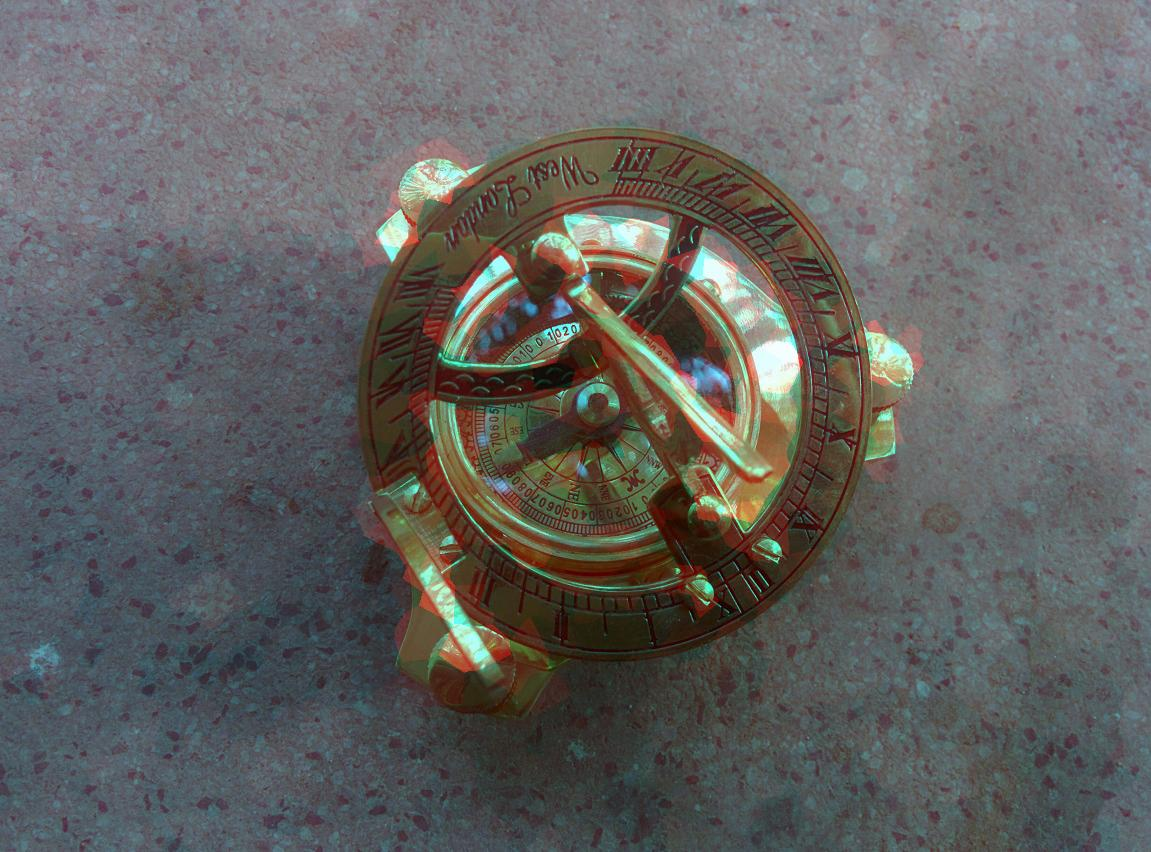
\includegraphics[width=\linewidth]{r_f_seed123.jpg}
\caption{channel=red, seed=123, fast}
\end{subfigure}
\begin{subfigure}[b]{0.48\linewidth}
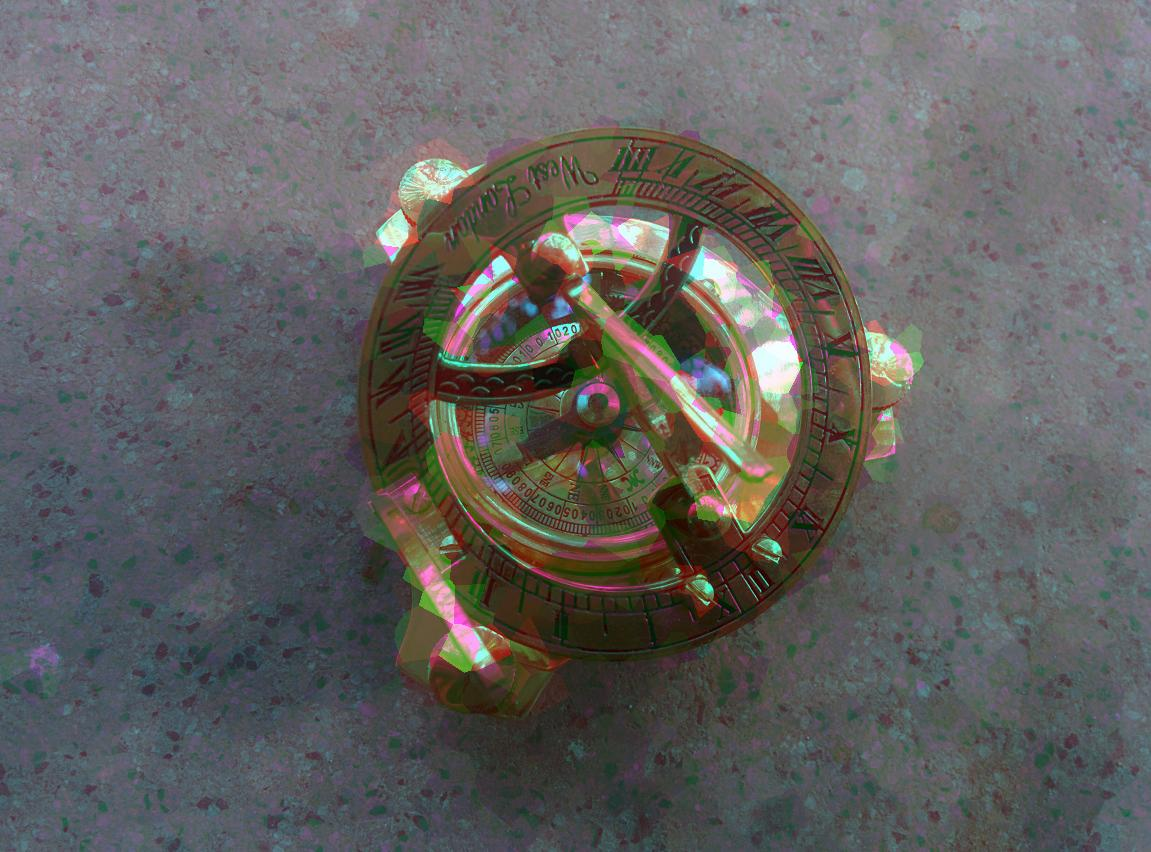
\includegraphics[width=\linewidth]{rand_f_seed123.jpg}
\caption{channel=rand, seed=123, fast}
\end{subfigure}
\end{figure}
\begin{figure}
\centering
\begin{subfigure}[b]{0.48\linewidth}
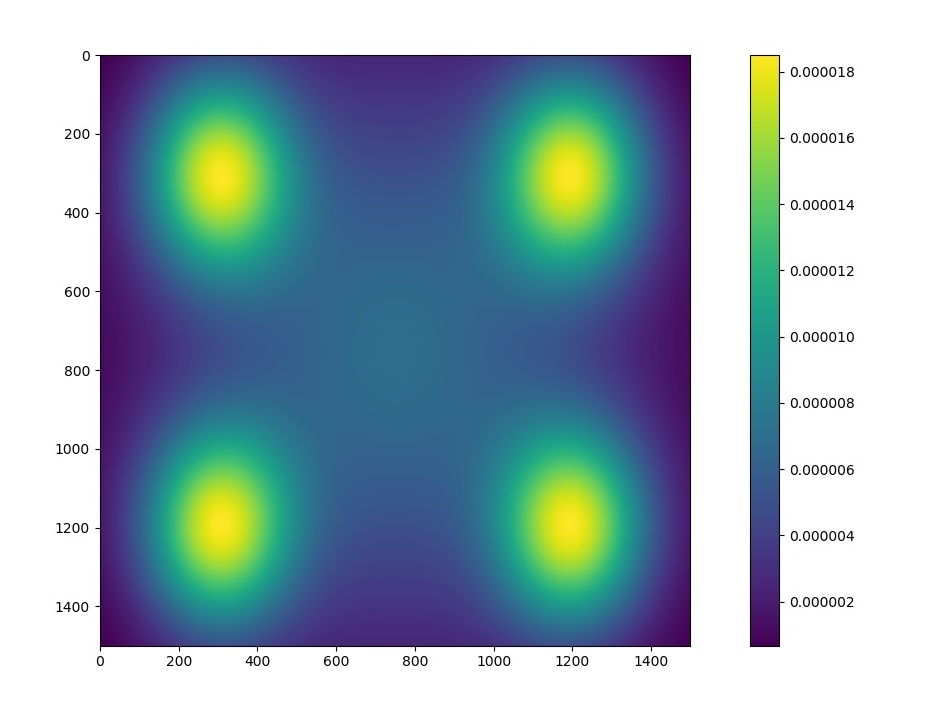
\includegraphics[width=\linewidth]{demo_probmap.jpg}
\caption{demo\_ probmap -heatmap}
\end{subfigure}
\begin{subfigure}[b]{0.48\linewidth}
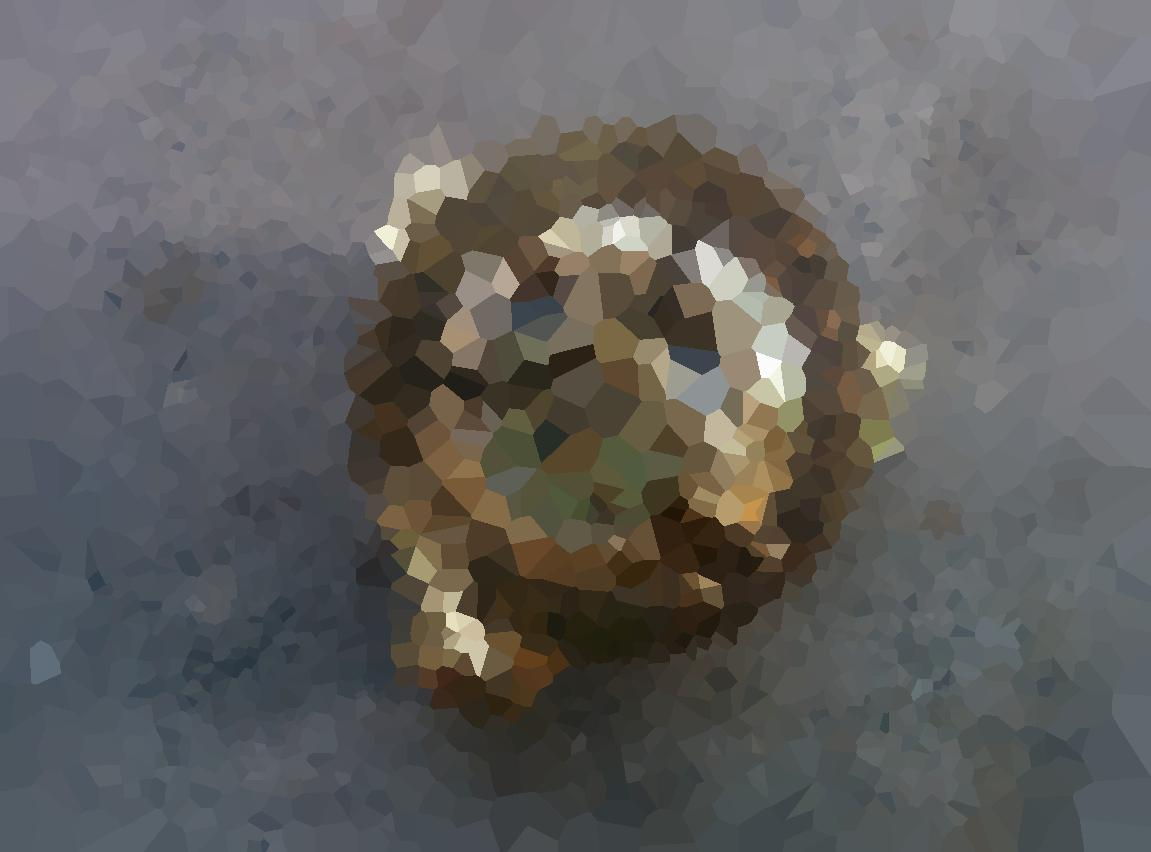
\includegraphics[width=\linewidth]{probmap_2500_f_seed123.jpg}
\caption{demo\_ probmap, seed=123, cn=2500, fast}
\end{subfigure}
\begin{subfigure}[b]{0.48\linewidth}
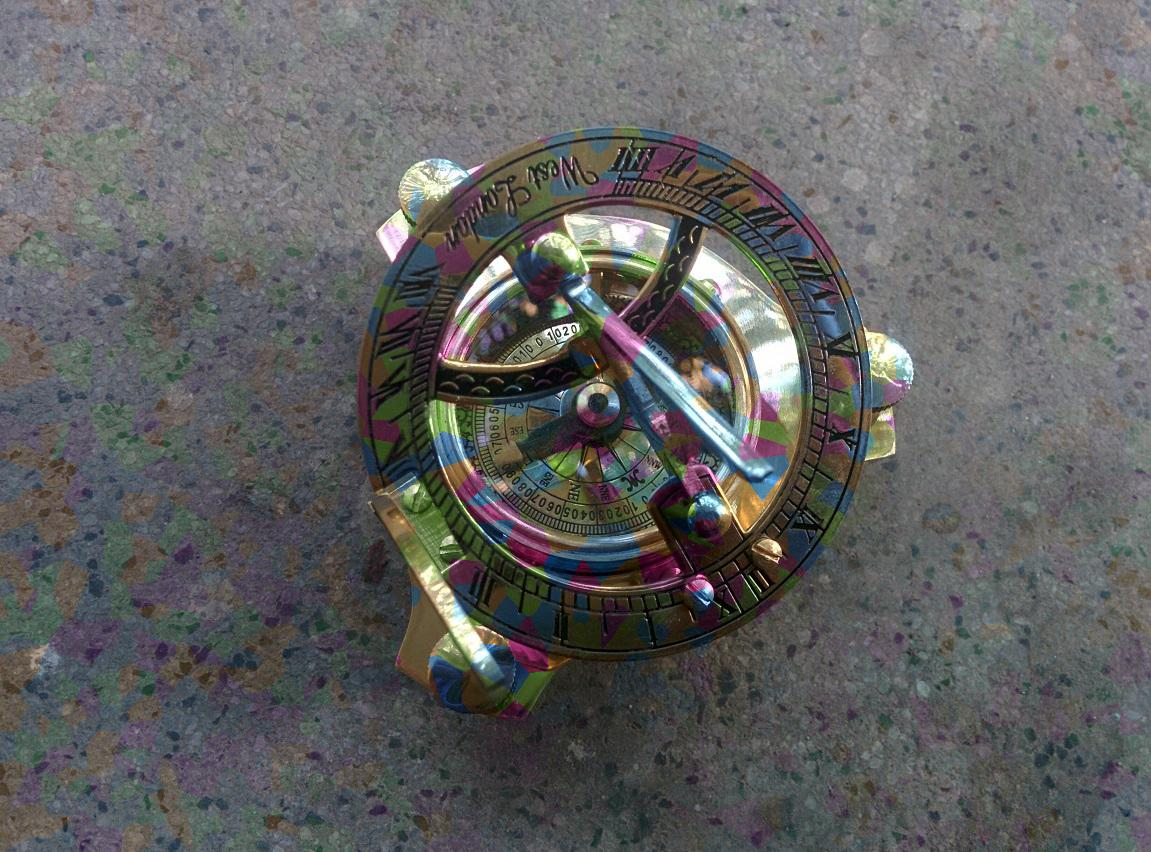
\includegraphics[width=\linewidth]{randdual_lm_seed123.jpg}
\caption{randdual, seed=123, low\_ mem}
\end{subfigure}
\begin{subfigure}[b]{0.48\linewidth}
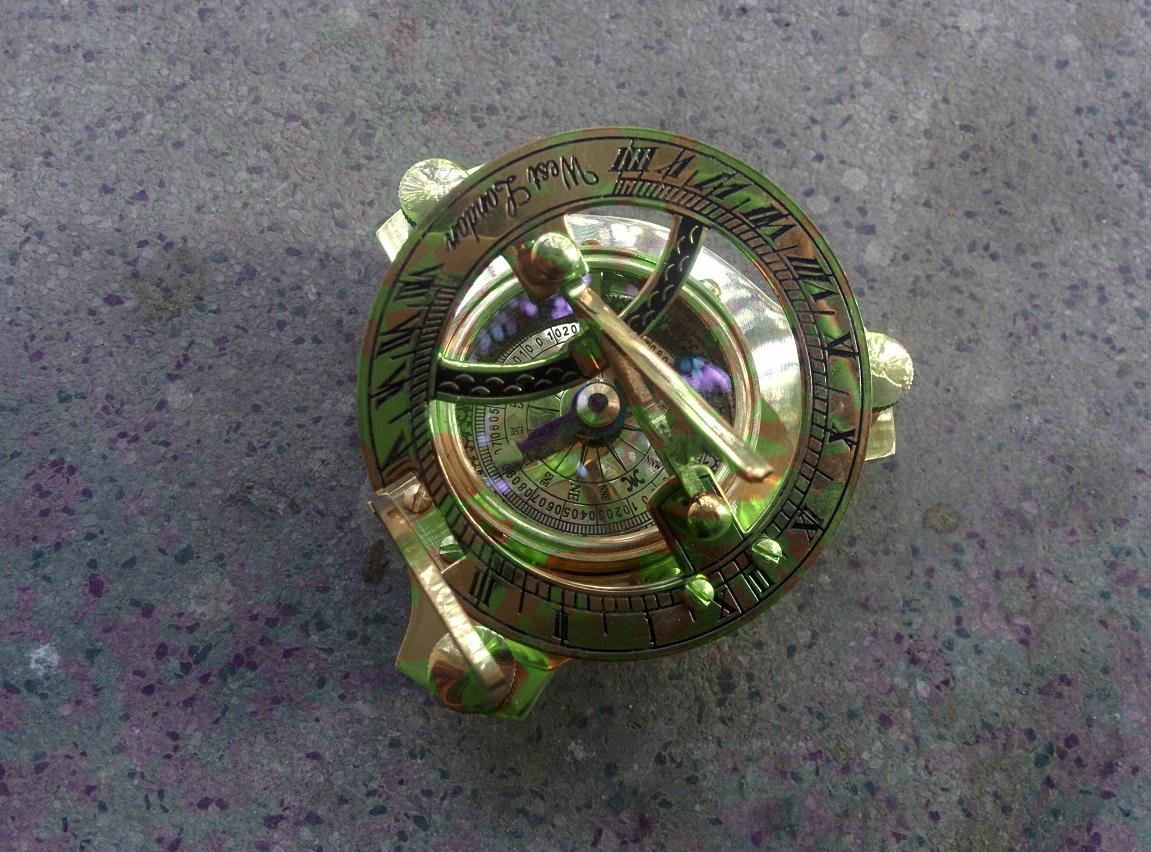
\includegraphics[width=\linewidth]{rg_lm_seed123.jpg}
\caption{channel=rg, seed=123, low\_ mem}
\end{subfigure}
\end{figure}
\end{document}